\chapter{Machine Learning}

\section{Frames Sampling}
To address the variable length of segments within the dataset, in instances where we aim to attain a lower number of frames than the actual length of the segments, 
we have utilized the \textit{uniform spacing} sampling technique to address the variability in segment lengths within the dataset.
This method entails selecting frames from a list or sequence at regular, even intervals. 
It proves to be highly advantageous when the goal is to ensure an equal distribution of frames throughout the sequence.

\begin{figure}[H]
    \centering
    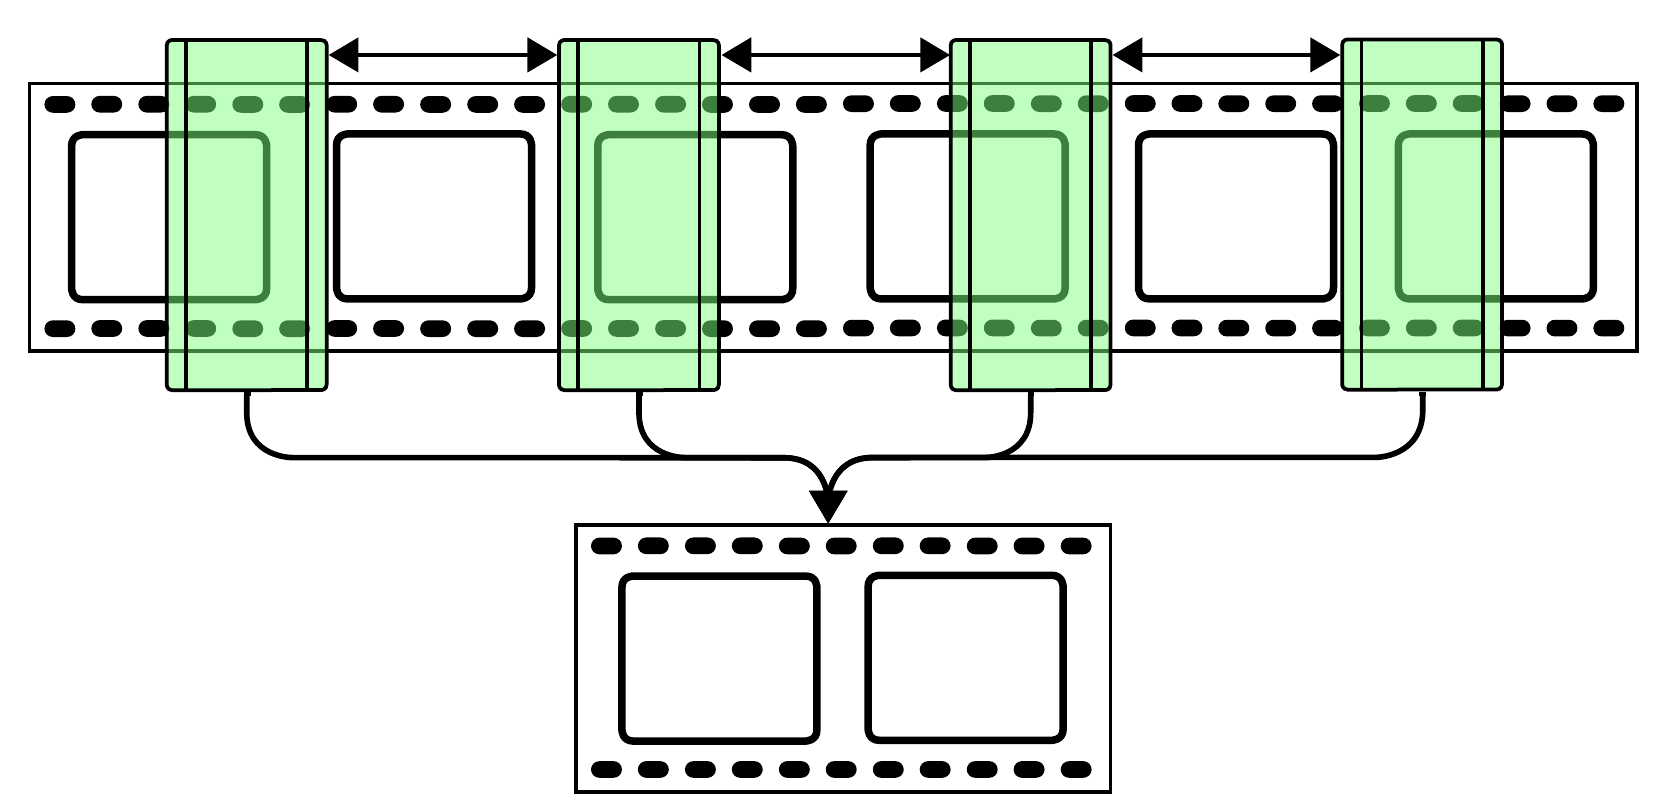
\includegraphics[width=0.8\textwidth]{graphics/subSampling.png}
    \caption{Uniform Sampling visualized}
    \label{fig:unif_sampling}
\end{figure}

Conversely, when dealing with segments that are shorter than the standard number of frames, a different technique is implemented.
In such cases, for each frame, a variable and uniform number of interpolation frames are inserted to reach the desired frame count. 
This approach compensates for the shorter segment length by adding interpolated frames, maintaining the consistency required for further analysis or processing.
\begin{figure}[H]
    \centering
    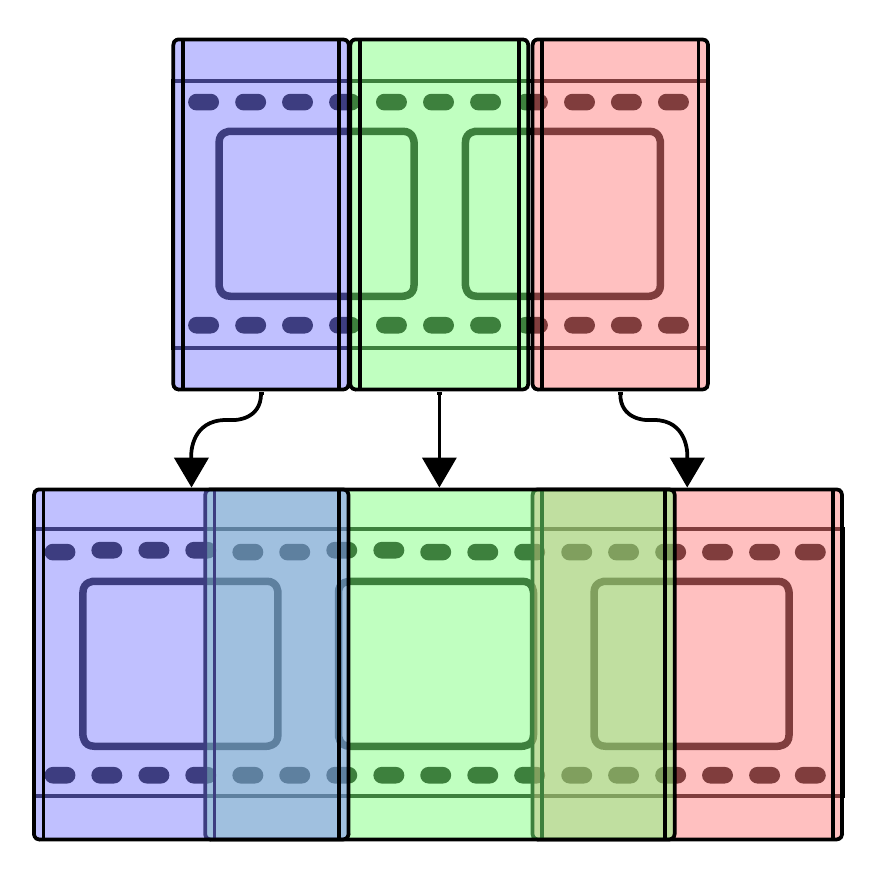
\includegraphics[width=0.4\textwidth]{graphics/interpolationSampling.png}
    \caption{Frames interpolation visualized}
    \label{fig:interp_sampling}
\end{figure}

\section{Dataset Normalization}
As previously mentioned, our dataset consists of 60 samples, each containing the spatial positions of all 20 skeletal joints at each time step.
From the equally sampled timeseries we calculate the $x$, $y$, and $z$ coordinates of the skeleton's barycenter for each time step. \\
We define the barycenter as the point where all the mass of an object or a system of objects is concentrated. \\
In this context, each joint is considered to have unit mass, meaning that all joints contribute equally to the barycenter. \\
If we represent $n$ as the number of 20 joints, the coordinates of the barycenter are obtained by taking the average of the coordinates of these 20 joints, as we can see in the formula:

\begin{equation}
    Barycenter (x, y, z) = \left(\frac{1}{n} \sum_{i=1}^{n} x_i, \frac{1}{n} \sum_{i=1}^{n} y_i, \frac{1}{n} \sum_{i=1}^{n} z_i\right)
    \label{formula:baricentro}
\end{equation}
    
where $x_i$, $y_i$, and $z_i$ represent the $x$, $y$, and $z$ coordinates of the $i$-th joint, respectively.

Subsequently, we calculate the distance between each joint and the barycenter, at each time step, using the Euclidean distance in Formula \ref{formula:distance}. \\
These distances from the barycenter will be normalized for each joint, in order to obtain normalized time series between 0 and 1.

\begin{equation}
    x_{norm} = \frac{{x - min(x)}}{{max(x) - min(x)}}
    \label{formula:normalization}
\end{equation}
    
The choice to calculate the distances between joints and the barycenter for each sample plays a crucial role in ensuring the robustness of our ML approach to variations in scale.
In scenarios where dancers or subjects may have different heights or body proportions, relying solely on absolute joint coordinates could introduce bias into the model.
However, by computing these distances and further normalizing them within the range of 0 to 1, we effectively eliminate the influence of scale variations.

This normalization process not only standardizes the data but also allows the ML model to focus on the relative spatial distribution of joints rather than their absolute positions.
Consequently, our model becomes better equipped to recognize patterns and movements across individuals of varying statures, making it more versatile and applicable in real-world scenarios. \\

\section{Features extraction}
Feature extraction in ML is an essential process that involves transforming raw data into a more suitable format for analysis and model building.
It helps identify and capture the most relevant information within the data while simplifying excessive complexity that could make model training challenging.
This process not only contributes to improving model accuracy but also reduces the risk of overfitting and enhances the ability to generalize knowledge gained to new data. \\
From the preprocessed data, we want to extract the necessary features for ML.
Here we will see al the steps involved in order to achieve the desired features, for every sample of the dataset (note that \textit{n} is the number of frames of the sample). \\
\begin{itemize}
    \item \textbf{Mean} is the expected value of the distribution:
        \begin{equation}
            mean(\bar{x}) = \frac{1}{n} \sum_{i=1}^{n} x_i
        \end{equation}
    \item \textbf{Variance} is the second momentum of the distribution (or the squared deviation of the expected value from the mean):
        \begin{align}
            mean_a(x) &= \frac{1}{n} \sum_{i=1}^{n} (x_i - mean(\bar{x}))^a &
            var(x) &= mean_2(\bar{x})
        \end{align}
    \item \textbf{Kurtosis} is the fourth standardized moment:
        \begin{equation}
            kurtosis(\bar{x}) = \frac{mean_4(\bar{x})}{\sqrt{var(\bar{x})}^4} - 3
        \end{equation}
    \item \textbf{Skewness} is the third standardized moment:
        \begin{equation}
            skewness(\bar{x}) = \frac{mean_3(\bar{x})}{\sqrt{var(\bar{x})}^3}
        \end{equation}
    \item \textbf{Correlation} between two joints (\textit{x},\textit{y}):
        \begin{equation}
            corr(\bar{x},\bar{y}) = \frac{\sum_{i=1}^n (x_i - mean(\bar{x}))(y_i - mean(\bar{y}))}{\sqrt{var(\bar{x})}\cdot\sqrt{var(\bar{y})}}
        \end{equation}
    \item \textbf{Mean Absolute Deviation}:
        \begin{equation}
            mad(\bar{x}) = \frac{1}{n} \sum_{i=1}^{n} |x_i - mean(\bar{x})|
        \end{equation}
    \item \textbf{Mean Standard Error}:
        \begin{equation}
            sem(\bar{x}) = \sqrt{\frac{var(\bar{x})}{n}}
        \end{equation}
    \item \textbf{Average Sum of Squares}:
        \begin{equation}
            energy(\bar{x}) = \sqrt{\sum_{i=1}^{n} x_i^2}
        \end{equation}
    \item \textbf{Interquantile Range} measures statistical dispersion in the range between the 25th (Q1) and the 75th percentile (Q3) of the data distribution ($ iqr = Q3 - Q1 $):
        \begin{equation}
            iqr(\bar{x}) =  
                \begin{cases} 
                \bar{x}_{\frac{3}{4}(n+1)} - \bar{x}_{(\frac{n+1}{4})} & \text{if n is odd} \\
                \frac{(\bar{x}_{(\frac{3}{4}n)} + \bar{x}_{(\frac{3}{4}n+1)}) - (\bar{x}_{(\frac{n}{4})} + \bar{x}_{(\frac{n}{4}+1)})}{2} & \text{otherwise}
                \end{cases}
        \end{equation}
        \begin{figure}[H]
            \centering
            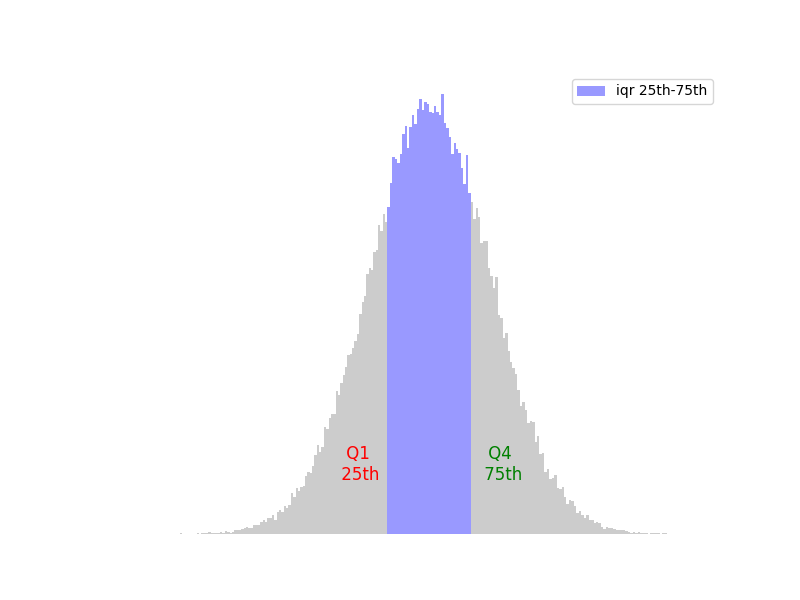
\includegraphics[width=0.85\textwidth]{graphics/iqr.png}
            \caption{Interquantile range of a normal distribution}
            \label{fig:iqr}
        \end{figure}
    \item \textbf{Fundamental Frequency Signal} from the Discrete Fourier Transform (DFT):
    \begin{equation}
        firstFreq(\bar{x}) = \angle DFT(\bar{x})[1]
    \end{equation}
    \item \textbf{Real part's Average of Frequency Signal}:
    \begin{equation}
        meanFreq(\bar{x}) = \sum_{i=1}^{n} Re(DFT(x_i))
    \end{equation}
    \item \textbf{Real part's Max of Frequency Signal}:
    \begin{equation}
        maxFreq(\bar{x}) = Max(Re(DFT(x)))
    \end{equation}
    \item \textbf{Index of the Max of the Real part of Frequency Signal}:
    \begin{equation}
        maxFreq(\bar{x}) = Argmax(Re(DFT(x)))
    \end{equation}
\end{itemize}
The last four values correspond to the minimum value and its index, skewness, and kurtosis of the Fourier transform.
To choose the features to extract, we referred to \cite{oneto:2020} and \cite{sama:2010}.
In Table \ref{tab:ml_features} we can see all the features and their relative function.

\begin{table}[H]
    \centering
    \begin{tabular}{|c|c|}
        \hline
        \textbf{Function} & \textbf{Description} \\
        \hline
        mean & Mean \\
        var & Variance \\
        kurtosis & Kurtosis \\
        skewness & Skewness \\
        corr & Correlation Coefficient \\
        mad & Mean Absolute Deviation \\
        sem & Mean Standard Error \\
        energy & Average Sum of Squares \\
        iqr & Interquantile Range \\
        min & Smallest Value in Array \\
        max & Largest Value in Array \\
        firstFreq & Fundamental Frequency Signal \\
        meanFreq & Real part's Average of Frequency Signal \\
        maxFreq & Real part's Max of Frequency Signal \\
        maxFreqIndx & Index of the Max of the Real part of Frequency Signal \\ 
        minFreq & Real part's Min of Frequency Signal \\
        minFreqIndx & Index of the Min of the Real part of Frequency Signal \\ 
        skewnessFreq & Frequency Signal Skewness \\
        kurtosisFreq & Frequency Signal Kurtosis \\
        \hline
    \end{tabular}
    \caption{List of measures for computing feature vectors}
\label{tab:ml_features}
\end{table}

\section{Method}

The initial approach to classification involves a straightforward binary classification of the origin of the movement within a specific edge.
If the results had been satisfactory, we would then have opted to evaluate progressively more complex models, eventually leading to the actual classification of the movement's origin from a video segment.

\subsection{Model creation}
We started by addressing the issue of imbalanced data in classification. Imbalanced data occurs when one class significantly outnumbers the other(s), leading to challenges in training a classifier that can effectively distinguish between the classes.
To mitigate this imbalance, a resampling technique known as B-SMOTE is employed (\textit{BS1}). The operational concept is detailed in Section \ref{subsec:borderline}.

Following the resampling of the training data, a RF classifier (\textit{RF1}) is trained on this newly balanced dataset.
To further optimize the classifier's performance, a feature selection process is employed with the goal of identifying the most influential features that contribute to accurate classification.
Initially, the most important features are determined through the training of \textit{RF1} on the resampled data. 
These crucial features are selected based on their significance in the classification task. 
Subsequently, a new RF classifier (\textit{RF2}) is trained using only the selected important features. 
To evaluate the performance of the classifier, a test set is chosen using LOOCV, as detailed in Section \ref{subsec:cross_validation}. 

\begin{table}[H]
    \centering
    \begin{tabular}{|c|c|c|}
        \hline
        \textbf{Model} & \textbf{Hyperparameter} & \textbf{Value} \\
        \hline
        \textit{BS1} & \textit{k}-\textit{neighbors} & 0.4 $\cdot$ count(Less Frequent Class)  \\
        & \textit{m}-\textit{neighbors} & 0.4 $\cdot$ count(Most Frequent Class)  \\
        \hline
        \textit{RF1} & \textit{n}\_\textit{estimators} & 500  \\
        & \textit{max}\_\textit{features} & Default  \\
        \hline
        \textit{RF2} & \textit{n}\_\textit{estimators} & 200  \\
        & \textit{max}\_\textit{features} & All  \\
        \hline
    \end{tabular}
    \caption{Hyperparameters tuned for our application}
    \label{tab:ml_param}
\end{table}

\subsection{Binary questions to the Model}
\label{sec:ml_bin_questions}
In our ML model, we posed three different questions regarding the OoM. 
Since our dataset is inherently a multi-class dataset, we performed binary classification by reclassifying the dataset.
These binary questions are posed either to edges or to specific parts of the skeleton, which are themselves composed of edges. \\
In Figures \ref{tab:ml_division_5_body_parts} and \ref{tab:ml_division_top_bottom}, you can observe which edges form various parts of the skeleton. \\
Note that not every edge of the reduced marker set (\ref{tab:labels_joints}) is included because some edges have not been the ground truth for any sample in our dataset.
For ML we have in total 15 classes, that is 15 edges.

\begin{table}[H]
    \centering
    \renewcommand{\arraystretch}{0.85}
    
    \begin{subtable}{\textwidth}
        \centering
        \begin{tabular}{|c|c|}
            \hline
            \textbf{Body Part} & \textbf{Edges} \\
            \hline
            Head & shoulder\_center - head \\
            \hline
            Right Arm & right\_hand - right\_wrist \\
            & right\_wrist - right\_elbow \\
            & right\_elbow - right\_shoulder \\
            & right\_shoulder - shoulder\_center \\
            \hline
            Left Arm & left\_hand - left\_wrist \\
            & left\_elbow - left\_shoulder \\
            & left\_shoulder - shoulder\_center \\
            \hline
            Right Leg & right\_foot - right\_ankle \\
            & right\_ankle - right\_knee \\
            & right\_knee - right\_hip \\
            & right\_hip - hip\_center \\
            \hline
            Left Leg & left\_foot - left\_ankle \\
            & left\_knee - left\_hip \\
            & left\_hip - hip\_center \\
            \hline
        \end{tabular}
        \caption{}
        \label{tab:ml_division_5_body_parts}
    \end{subtable}

    \vspace{10pt} % Add vertical space between subtables

    \begin{subtable}{\textwidth}
        \centering
        \begin{tabular}{|c|c|}
            \hline
            \textbf{Body Part} & \textbf{Edges} \\
            \hline
            Upper & right\_hand - right\_wrist \\
            & right\_wrist - right\_elbow \\
            & right\_elbow - right\_shoulder \\
            & right\_shoulder - shoulder\_center \\
            & left\_hand - left\_wrist \\
            & left\_elbow - left\_shoulder \\
            & left\_shoulder - shoulder\_center \\
            & shoulder\_center - head \\
            \hline
            Lower & right\_foot - right\_ankle \\
            & right\_ankle - right\_knee \\
            & right\_knee - right\_hip \\
            & right\_hip - hip\_center \\
            & left\_foot - left\_ankle \\
            & left\_knee - left\_hip \\
            & left\_hip - hip\_center \\
            \hline
        \end{tabular}
        \caption{}
        \label{tab:ml_division_top_bottom}
    \end{subtable}

    \caption{Skeleton Division in 5 parts (a) and in 2 parts (b)}
    \label{tab:ml_skeleton_divisions}
\end{table}

The Q1 will be posed considering the 15 edges, the Q2 will be posed considering the division of the body into 5 parts (Figure \ref{tab:ml_division_5_body_parts}), while Q3 will be based on the division of the body into 2 parts (Figure \ref{tab:ml_division_top_bottom}).


\begin{itemize}

    \item \textbf{(Q1) Is or is not a specific edge:} In our dataset, the most frequent classification is the edge that links \textit{left\_hand} and \textit{left\_wrist}. 
    Therefore, we categorized all samples where the classification was \textit{left\_hand}-\textit{left\_wrist} as 1, while we labeled all other samples as 0.   
    
    \item \textbf{(Q2) Is or is not a specific body part:} The most frequent class to compare against all the others is \textit{Right Leg}.
    Therefore, we labeled all samples where the classification was in the \textit{Right Leg} as 1, while we categorized all other samples as 0.

    \item \textbf{(Q3) Is or is not a specific body part:} The most frequent class between the two is \textit{Upper}, so we labeled all the $Upper$ with 1 and all the $Lower$ with 0.
    
   
\end{itemize}

For each question, we iteratively asked the model whether the test sample was predicted as that edge/that part of the body or not.

\section{Results}
In the following Tables (from \ref{tab:ml_results_cm_joints} to \ref{tab:ml_results_cm_body_parts}), you will find confusion matrices and evaluation metrics for the prediction of certain classes.
To interpret the meaning of the confusion matrices, please refer to Section \ref{subsec:evaluation_metrics}.
\\

The tests to identify the best model were conducted on the most frequent edge of the dataset, \textit{left\_hand - left\_wrist} with the aim of maximize the accuracy.
This is because the dataset is unbalanced, and therefore, better prediction results are expected from this class.
As observed, accuracy consistently remains very high, almost always exceeding 70\%.
However, beyond this, the model demonstrates high $specificity$, meaning it excels at maximizing TN but struggles to identify TP effectively.
This behavior is evident in the TPR, which varies significantly across different classes.
The model requires a high level of certainty in predictions before classifying a sample as positive.
You can also observe the model's high specificity from the TNR, which is consistently quite high in all cases, typically greater than 80\%. \\
In summary, the model tends to favor a conservative strategy, prioritizing the reduction of FP, leading to a high specificity but limited effectiveness in identifying TP.


\begin{table}[H]
    \centering
    \renewcommand{\arraystretch}{1.2} % Aumenta lo spazio tra le righe del doppio
    \begin{subfigure}[b]{0.1\textwidth}
        \centering
        \begin{tabular}{|>{\centering\arraybackslash}p{0.5cm}|>{\centering\arraybackslash}p{0.5cm}|}
        \hline
        48 & 3 \\
        \hline
        3 & 6 \\
        \hline
        \end{tabular}
        \caption{}
        \label{tab:ml_results_cm_edge_1}
    \end{subfigure}
    \hspace{0.05\linewidth}
    \begin{subfigure}[b]{0.1\textwidth}
        \centering
        \begin{tabular}{|>{\centering\arraybackslash}p{0.5cm}|>{\centering\arraybackslash}p{0.5cm}|}
        \hline
        51 & 2 \\
        \hline
        6 & 1 \\
        \hline
        \end{tabular}
        \caption{}
        \label{tab:ml_results_cm_edge_2}
    \end{subfigure}
    \hspace{0.05\linewidth}
    \begin{subfigure}[b]{0.1\textwidth}
        \centering
        \begin{tabular}{|>{\centering\arraybackslash}p{0.5cm}|>{\centering\arraybackslash}p{0.5cm}|}
        \hline
        44 & 9 \\
        \hline
        7 & 0 \\
        \hline
        \end{tabular}
        \caption{}
        \label{tab:ml_results_cm_edge_3}
    \end{subfigure}
    \hspace{0.05\linewidth}
    \begin{subfigure}[b]{0.1\textwidth}
        \centering
        \begin{tabular}{|>{\centering\arraybackslash}p{0.5cm}|>{\centering\arraybackslash}p{0.5cm}|}
        \hline
        51 & 3 \\
        \hline
        4 & 2\\
        \hline
        \end{tabular}
        \caption{}
        \label{tab:ml_results_cm_edge_4}
    \end{subfigure}
    \hspace{0.05\linewidth}
    \begin{subfigure}[b]{0.1\textwidth}
        \centering
        \begin{tabular}{|>{\centering\arraybackslash}p{0.5cm}|>{\centering\arraybackslash}p{0.5cm}|}
        \hline
        52 & 3 \\
        \hline
        4 & 1 \\
        \hline
        \end{tabular}
        \caption{}
        \label{tab:ml_results_cm_edge_5}
    \end{subfigure}
    \hspace{0.05\linewidth}
    \begin{subfigure}[b]{0.1\textwidth}
        \centering
        \begin{tabular}{|>{\centering\arraybackslash}p{0.5cm}|>{\centering\arraybackslash}p{0.5cm}|}
        \hline
        53 & 2 \\
        \hline
        2 & 3 \\
        \hline
        \end{tabular}
        \caption{}
        \label{tab:ml_results_cm_edge_6}
    \end{subfigure}
    \hspace{0.05\linewidth}
    \caption{Confusion matrices of the 6 most frequent classes in the dataset}
    \label{tab:ml_results_cm_joints}
\end{table}

%TODO AGGIUNGERE TOP FEATURES PER EXPLAINABILITY
\begin{table}[H]
    \centering
    \begin{tabular}{|>{\centering\arraybackslash}p{2cm}|>{\centering\arraybackslash}p{6cm}|>{\centering\arraybackslash}p{2cm}|>{\centering\arraybackslash}p{2cm}|>{\centering\arraybackslash}p{2cm}|}
    \hline
    \textbf{Label} & \textbf{Edge} & \textbf{TPR} & \textbf{TNR} &\textbf{Accuracy} \\
    \hline
    (a) & left\_hand - left\_wrist  & 66\% & 94\% & 90\% \\
    \hline
    (b) & shoulder\_center - head  & 14\% & 96\% & 87\% \\
    \hline
    (c) & right\_elbow - right\_shoulder  & 0\%  & 83\% & 73\% \\ 
    \hline
    (d) & right\_shoulder - shoulder\_center & 33\% & 94\% & 88\% \\
    \hline
    (e) & right\_knee - right\_hip  & 20\%  & 95\% & 88\%\\
    \hline
    (f) & left\_knee - left\_hip  & 60\% & 96\% & 93\%\\ 
    \hline
    \end{tabular}
    \caption{Metrics of the 6 classes most frequent of the dataset}
    \label{tab:ml_results_joints}
\end{table}




\begin{table}[H]
  \begin{minipage}[b]{0.1\textwidth}
    \centering
    \renewcommand{\arraystretch}{1.2} % Aumenta lo spazio tra le righe del doppio
    \begin{tabular}{|>{\centering\arraybackslash}p{0.5cm}|>{\centering\arraybackslash}p{0.5cm}|}
    \hline
    37 & 5 \\
    \hline
    7 & 11 \\
    \hline
    \end{tabular}
    \caption*{(g)}
    \label{tab:ml_results_cm_body_part_1}
  \end{minipage}
  \hspace{0.05\linewidth}
  \begin{minipage}[b]{0.1\textwidth}
    \centering
    \renewcommand{\arraystretch}{1.2} % Aumenta lo spazio tra le righe del doppio
    \begin{tabular}{|>{\centering\arraybackslash}p{0.5cm}|>{\centering\arraybackslash}p{0.5cm}|}
    \hline
    37 & 9 \\
    \hline
    10 & 4 \\
    \hline
    \end{tabular}
    \caption*{(h)}
    \label{tab:ml_results_cm_body_part_2}
  \end{minipage}
  \hspace{0.05\linewidth}
  \begin{minipage}[b]{0.1\textwidth}
    \centering
    \renewcommand{\arraystretch}{1.2} % Aumenta lo spazio tra le righe del doppio
    \begin{tabular}{|>{\centering\arraybackslash}p{0.5cm}|>{\centering\arraybackslash}p{0.5cm}|}
    \hline
    43 & 4 \\
    \hline
    6 & 7 \\
    \hline
    \end{tabular}
    \caption*{(i)}
    \label{tab:ml_results_cm_body_part_3}
  \end{minipage}
  \hspace{0.05\linewidth}
  \begin{minipage}[b]{0.1\textwidth}
    \centering
    \renewcommand{\arraystretch}{1.2} % Aumenta lo spazio tra le righe del doppio
    \begin{tabular}{|>{\centering\arraybackslash}p{0.5cm}|>{\centering\arraybackslash}p{0.5cm}|}
    \hline
    47 & 5 \\
    \hline
    7 & 1\\
    \hline
    \end{tabular}
    \caption*{(l)}
    \label{tab:ml_results_cm_body_part_4}
  \end{minipage}
  \hspace{0.05\linewidth}
  \begin{minipage}[b]{0.1\textwidth}
    \centering
    \renewcommand{\arraystretch}{1.2} % Aumenta lo spazio tra le righe del doppio
    \begin{tabular}{|>{\centering\arraybackslash}p{0.5cm}|>{\centering\arraybackslash}p{0.5cm}|}
    \hline
    51 & 2 \\
    \hline
    6 & 1 \\
    \hline
    \end{tabular}
    \caption*{(m)}
    \label{tab:ml_results_cm_body_part_5}
  \end{minipage}
  \hspace{0.05\linewidth}
  \begin{minipage}[b]{0.1\textwidth}
    \centering
    \renewcommand{\arraystretch}{1.2} % Aumenta lo spazio tra le righe del doppio
    \begin{tabular}{|>{\centering\arraybackslash}p{0.5cm}|>{\centering\arraybackslash}p{0.5cm}|}
        \hline
        16 & 5 \\
        \hline
        8 & 31 \\
        \hline
    \end{tabular}
    \caption*{(n)}
    \label{tab:ml_results_cm_body_part_6}
  \end{minipage}
  \hfill
  \caption{Confusion matrices of the 5 Body Parts classification and of the Upper/Lower one}
  \label{tab:ml_results_cm_body_parts}
\end{table}


\begin{table}[H]
    \centering
    \begin{tabular}{|>{\centering\arraybackslash}p{2cm}|>{\centering\arraybackslash}p{6cm}|>{\centering\arraybackslash}p{2cm}|>{\centering\arraybackslash}p{2cm}|>{\centering\arraybackslash}p{2cm}|}
        \hline
        \textbf{Label} & \textbf{Body Part} & \textbf{TPR} & \textbf{TNR} & \textbf{Accuracy} \\
        \hline
        (g) & Right Arm  & 61\% & 88\% & 80\% \\
        \hline
        (h) & Left Arm & 29\% & 80\% & 68\% \\
        \hline
        (i) & Right Leg  & 54\%  & 91\% & 83\% \\ 
        \hline
        (l) & Left Leg & 12\% & 90\% & 80\% \\
        \hline
        (m) & Head  & 14\%  & 96\% & 86\%\\
        \hline
    \end{tabular}
    \begin{tabular}{|>{\centering\arraybackslash}p{2cm}|>{\centering\arraybackslash}p{6cm}|>{\centering\arraybackslash}p{2cm}|>{\centering\arraybackslash}p{2cm}|>{\centering\arraybackslash}p{2cm}|}
        \hline
        \textbf{Label} & \textbf{Body Half} & \textbf{TPR} & \textbf{TNR} & \textbf{Accuracy} \\
        \hline
        (n) & Upper & 79\% & 76\% & 78\% \\
        \hline
    \end{tabular}
    \caption{Metrics of the 5 Body Parts and the Upper}
    \label{tab:ml_results_body_parts}
\end{table}
